\chapter{Implementierung}
\label{sec:implementierung}
Dieses Kapitel beschreibt die Implementierung der zuvor konzipierten Webanwendung anhand einiger Codebeispiele. Zunächst werden die verwendeten Webtechnologien vorgestellt. Danach folgt der Abschnitt Datenmodellierung. In diesem werden das Datenbankschema und die Datenbankstruktur, welche durch ein ER-Modell festgelegt wird, dargestellt. Weiter geht es mit der Architektur und Struktur der Webanwendung. Dabei wird in diesem Abschnitt das MVC-Entwurfsmuster behandelt. Anschließend wird die eigentliche Implementierung, welche in serverseitig und clientseitig aufgeteilt sind, beschrieben.

\section{Verwendete Webtechnologien}
\label{sec:verwendete webtechnologien}
In diesem Unterkapitel werden die verwendeten Webtechnologien erläutert. 

\subsection{MidCom CMS}
\label{subsec:midcom cms}
Symfony\footnote{\url{https://symfony.com/}} ist eines der weltweit größten PHP Frameworks und wird von führenden Open-Source Projekten eingesetzt, wie zum Beispiel Drupal oder Wordpress. Das hauseigene Webframework MidCom CMS basiert auf der Symfony Umgebung, dies gibt die Architektur einer Webanwendung vor und stellt eine Vielzahl an fertig implementierten Modulen bereit, die den Programmieraufwand reduzieren.

\subsection{HTML - Hypertext Markup Language}
\label{subsec:html}
\par
\begingroup
\leftskip=4em % Parameter anpassen
\rightskip\leftskip
\noindent \glqq Webseiten bestehen erst einmal aus reinem Text. Eine HTML-Seite wird nicht programmiert, es gibt keine Funktionen, die bei der Erfüllung bestimmter Bedingungen ausgeführt werden, wie das berühmte if-else in Programmiersprachen. Für eine Webseite wird erst einmal ein Text geschrieben und dieser Text wird dann mit HTML kodiert, das heißt, die logischen Bestandteile eines textorientierten Dokuments werden beschrieben. Dadurch werden die einzelnen Bestandteile des Textes zu HTML-Elementen (wie Überschriften, Absätze, List usw.). HTML beschreibt nicht, wie ein Element aussieht oder wo es platziert ist, HTML beschreibt, was ein Element ist - eine Überschrift, eine Liste, ein Bild, eine Tabelle usw. Es geht einzig und allein um die Struktur eines Dokuments, nicht um seine Präsentation\grqq{} \cite{Schu2008}
\par
\endgroup
\bigskip

HTML ist der grundlegende Bestandteil einer Webseite. Es verwendet “Markup” (Begriff für Textauszeichnung), um ein Dokument semantisch zu strukturieren. Um die Auszeichnung des Contents auf dem Webbrowser darzustellen, werden Markup-Elemente, so genannte Tags, verwendet. Diese Elemente sind innerhalb einer Auszeichnungssprache wie HTML standardisiert. Tags werden in spitzen Klammern notiert. Der Inhalt wird durch ein einleitendes und ein abschließendes Tag markiert.

\subsection{CSS - Cascading Styesheets}
\label{subsec:css}
\par
\begingroup
\leftskip=4em % Parameter anpassen
\rightskip\leftskip
\noindent \glqq Cascading Stylesheets (CSS) sind die Formatierungssprache für Webseiten. Der Einsatz von CSS bietet viele Vorteile, denn CSS ermöglicht eine Trennung von Inhalt und Layout: Damit lassen sich per CSS gestaltete Webseiten besser warten und leichter aktualisieren. Möchten Sie beispielsweise alle Überschriften eines Webprojekts in einer anderen Farbe ausgeben lassen, so müssen Sie bei einem konsequenten Einsatz von CSS die Änderung nur an einer Stelle, in einer von den (X)HTML-Dateien separaten Datei, vornehmen. Wird diese Formatierung hingegen direkt in (X)HTML realisiert, sind Änderungen bei jeder einzelnen Überschrift in den Dateien selbst durchzuführen.\grqq{} \cite{WHM2011}
\par
\endgroup
\bigskip

Während HTML den Aufbau bzw. die Struktur der Webseite bestimmt, ist CSS für das Aussehen der Elemente zuständig.

\subsection{Bootstrap}
\label{subsec:bootstrap}
Um ein einheitliches Erscheinungsbild für die Webanwendung zu erhalten, verwende ich das kostenlose und quelloffene Frontend-Framework namens Bootstrap.
Das Framework stellt verschiedene HTML- und CSS-Gestaltungsvorl\-agen für Formulare, Buttons, Tabellen, Navigation, Typografie sowie das Grid-System für Layouts zur Verfügung. Durch ein JavaScript-Modul ist es möglich, die Interaktionen auf der Webanwendung einzubinden. Außerdem bietet Bootstrap alle Voraussetzungen für ein responsives Webdesign, um die Webanwendung auf allen Geräten (Desktop, Smartphone und Tablet) einheitlich und optimal darzustellen.

\subsection{PHP - Hypertext Preprocessor}
\label{subsec:php}
PHP ist eine weit verbreitete Programmiersprache speziell für die Entwicklung dynamischer Webanwendungen. PHP ist plattformübergreifend und lässt sich in HTML einbinden. Anders als JavaScript ist PHP eine serverseitige Programmiersprache. Demzufolge läuft der PHP-Code auf dem Server und die fertige Webseite wird vom Server an den Benutzer ausgeliefert. Die ausgelieferte Webseite enthält keinen Programmiercode, sondern nur HTML-Code, welcher vom Browser verarbeitet und dargestellt wird.\footnote{vgl. \url{https://www.php.net/manual/de/intro-whatis.php}}

\subsection{phpMyAdmin}
\label{subsec:phpMyAdmin}
phpMyAdmin ist eine kostenlose Software für das Verwalten von MySQL-Datenbanken. Es werden Datenbanken zur Verfügung gestellt, in denen Inhalte in Tabellen abgespeichert werden. phpMyAdmin stellt eine grafische Benutzeroberfläche bereit, um Datenbanken ohne MySQL-Kenntnisse zu verwalten.

\subsection{JQuery UI}
\label{subsec:JQuery UI}
JQuery UI ist die Erweiterung von JQuery (\textbf{Abschnitt \ref{sec:jQuery}}) und bietet unabhängig vom Webbrowser die Funktionalität zur Gestaltung interaktiver Benutzeroberflächen. (vgl. \cite{Ste2019})\bigskip

Unter anderem stellt JQuery UI folgende Interaktionen zur Verfügung:
\begin{itemize}
\item Sortable: Einträge innerhalb einer Liste sortieren.
\item Draggable: Elemente innerhalb eines Bereiches verschieben.
\item Droppable: Elemente verschieben und ablegen, wie Drag \& Drop.
\item Selectable: Ein Element oder mehrere Elemente selektieren.
\end{itemize}

Um die Daten auf der Präsentation-Seite in Kategorien zusammenfassen zu können, wird dafür die Funktion \glqq Sortable\grqq{} angewendet.

\subsection{Ratchet und Autobahn|JS}
\label{subsce:Ratchet und Autobahn|JS}
\begin{itemize}
\item \textbf{Ratchet - WebSockets for PHP:}\\
Bei Ratchet\footnote{\url{http://socketo.me/docs/}} handelt es sich um eine PHP-Bibliothek für eine WebSocket-Anwendung. WebSocket ist eine bidirektionale und vollduplexe Kommunikation zwischen einem Webbrowser und Server \textbf{(Abschnitt \ref{sec:websocket})}.\bigskip

\begin{figure}[H]
  \begin{center}
    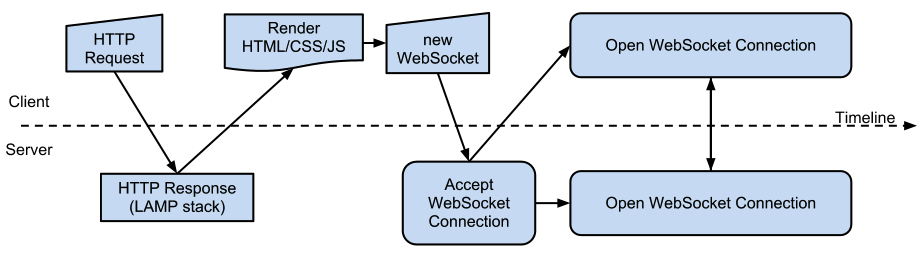
\includegraphics[scale=0.4]{img/RatchetFlow}
	\caption{Ratchet-Workflow} 
	\footnotesize\sffamily\textbf{Quelle:} \url{http://socketo.me/docs/flow}  
	\label{fig:ratchet-workflow}
  \end{center}   
\end{figure}

Sobald eine WebSocket-Verbindung erfolgreich aufgebaut ist, können Server und Client gleichzeitig miteinander kommunizieren.

\item \textbf{Autobahn|JS:}\\
Autobahn|JS ist ein Teilprojekt von Autobahn Projekt\footnote{\url{https://crossbar.io/autobahn/}} und bietet eine Open-Source Implementierung von Web Application Messaging Protocol\footnote{url{https://github.com/crossbario/autobahn-js}} (WAMP) in JavaScript.
\end{itemize}

Für die Umsetzung der Webanwendung werden sowohl Ratchet als auch Autobahn|JS zum Einsatz kommen. Ratchet wird als WebSocket-Server verwendet und Autobahn|JS als Client, der mit dem Ratchet kommuniziert.

\section{Datenmodellierung}
\label{sec:Datenmodellierung}
Ein gut strukturierter Datenbestand in Form einer relationalen Datenbank ist die Grundvoraussetzung der zu realisierenden Webanwendung. Als Werkzeug für die Verwaltung von Datenbanken kommt das freie Administration-Backend phpMyAdmin \textbf{(Abschnitt \ref{subsec:phpMyAdmin})} zum Einsatz. Als erster Schritt der Datenmodellierung wird die Datenbankstruktur mit einem ER-Modell festgelegt. Durch ein ER-Modell kann eine Datenbankstruktur vor der Programmierung geplant und verbessert werden. 

\subsection{ER-Modell}
\label{subsec:ER-Modell}
Ein ER-Modell besteht grob aus drei Teilen:
\begin{itemize}
\item \textbf{Entität:}\\
Objekte aus der realen Welt und gleichzeitig der Tabellenname.
\item \textbf{Attribut:}\\
Eigenschaft der Entität. Das entspricht der Spalte in der Tabelle. Ein Attribut besteht aus einfachen Datentypen wie integer oder char.
\item \textbf{Beziehung:}\\
Beziehung zwischen Entitäten. Dabei gibt es 1:1, 1:n und n:m Beziehungen.
\end{itemize}

\newpage
Die \textbf{Abbildung \ref{fig:ER-Modell}} visualisiert die Datenbanktabellen. Aus Gründen der Übersichtlichkeit wird bewusst auf die Darstellung der Attribute verzichtet.\bigskip

\begin{figure}[H]
  \begin{center}
    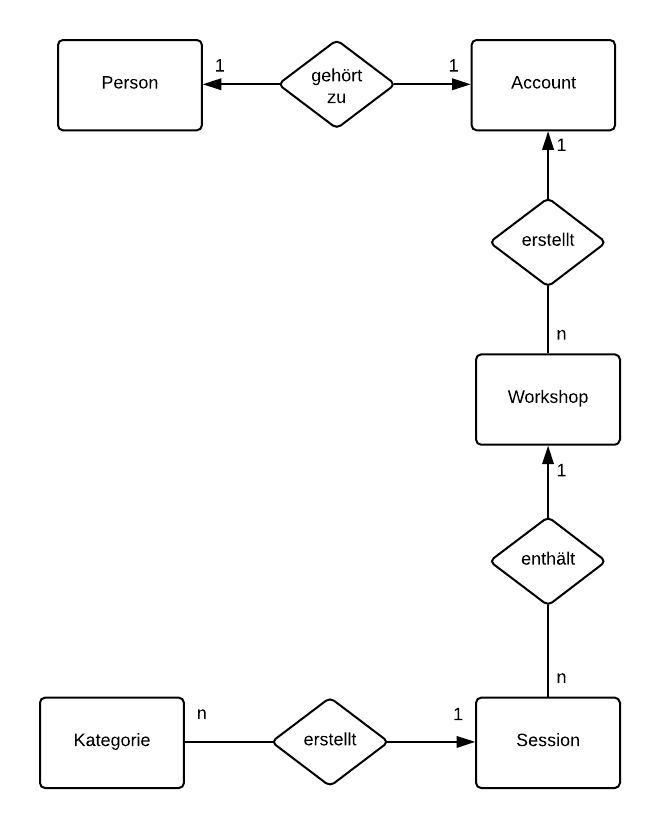
\includegraphics[scale=0.8]{img/erModell}
	\caption{ER-Modell der Webanwendung} 
	\footnotesize\sffamily\textbf{Quelle:} eigene Abbildung  
	\label{fig:ER-Modell}
  \end{center}   
\end{figure}

Eine Person gehört genau zu einem User-Account und ein User-Account gehört zu einer Person. Ein User-Account kann mehrere Workshops erstellen, aber ein Workshop kann höchsten von einem User-Account erstellt werden. Ein Workshop kann mehrere Sessions enthalten, wobei eine Session von genau einem Workshop zugeordnet wird. In einer Session können mehrere Kategorien erstellt werden, aber eine Kategorie wird höchstens von einer Session erstellt. 

\newpage
\subsection{Datenbankschema}
\label{subsec:Datenbankschema}
Vom ER-Modell \textbf{(Abbildung \ref{fig:ER-Modell})} wird das Datenbankschema abgeleitet. Die \textbf{Abbildung \ref{fig:datenbankschema}} gibt eine Übersicht über die einzelnen Tabellen mit ihren Attributen sowie die Beziehungen. Für die Durchführung von Workshops werden drei Tabellen (workshop, session und category) benötigt. Der User-Account wird in die midgard\_user-Datenbank gespeichert, welche in einer Beziehung zu der Person-Tabelle steht.\bigskip

\begin{figure}[H]
  \begin{center}
    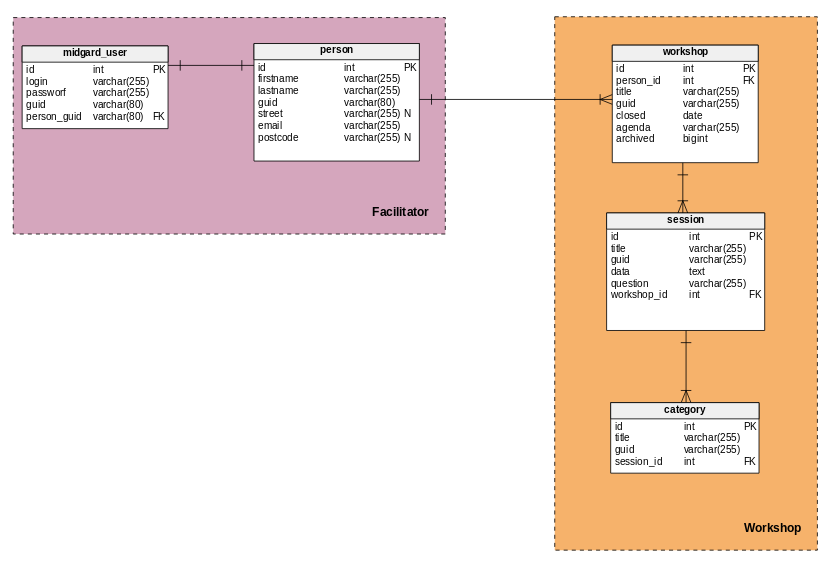
\includegraphics[scale=0.45]{img/datenbankschema}
	\caption{Datenbankschema} 
	\footnotesize\sffamily\textbf{Quelle:} eigene Abbildung  
	\label{fig:datenbankschema}
  \end{center}   
\end{figure}

\newpage
\section{Architektur der Webanwendung}
\label{sec:Architektur der Webanwendung}
Die Architektur der zu entwickelnden Webanwendung ist angelehnt an das \textbf{Model-View-Controller (MVC)} Entwurfsmuster. Daher wird dieses in diesem Unterkapitel erläutert und dargestellt.\bigskip

\par
\begingroup
\leftskip=4em % Parameter anpassen
\rightskip\leftskip
\noindent \glqq Das MVC-Konzept wurde 1979 zunächst für Benutzeroberflächen in Smalltalk durch Trygve Reenskaug beschrieben (Seeheim-Modell), der damals an Smalltalk im Xerox PARC arbeitete. Es gilt mittlerweile aber als De-facto-Standard für den Grobentwurf vieler komplexer Softwaresysteme, teils mit Differenzierungen und oftmals mehreren jeweils nach dem MVC-Muster aufgeteilten Modulen.\grqq{} \cite{Wiki2019d}
\par
\endgroup
\bigskip

Das Ziel dieses Entwurfsmusters ist es, eine interaktive Anwendung in drei Komponenten mit unterschiedlichen Aufgaben zu unterteilen. (vgl. \cite{Frank1996})

\begin{itemize}
\item \textbf{Model (M)}\\
Das Model enthält die Anwendungsdaten, die dem Benutzer mithilfe der View repräsentiert werden. Bei einer Änderung des Models werden alle zugehörigen View über die Änderung benachrichtigt, so dass die Daten auch auf der View-Komponente aktualisiert werden.
\item \textbf{View (V)}\\
Die View stellt dem Benutzer die Daten aus dem Model dar. Für das Model kann es mehrere Views geben. Dies hat vor allem den Vorteil, dass die Views andere Ausgaben generieren können.
\item \textbf{Controller (C)}\\
Der Controller ist sowohl mit der View als auch mit dem Model verbunden. Sie reagiert auf Benutzeraktionen, manipuliert sie im Model und aktualisiert selbst in einigen Fällen auch die View. Jede Veränderung von Daten informiert der Controller dem Model und das Model wiederum setzt die View über die Datenänderung in Kenntnis, so dass die Daten aktualisiert werden können.
\end{itemize}

\newpage
Die \textbf{Abbildung \ref{fig:mvc}} stellt grafisch die Kommunikationsverbindung der drei Komponenten in einem MVC-Entwurfs\-muster dar.\bigskip

\begin{figure}[H]
  \begin{center}
    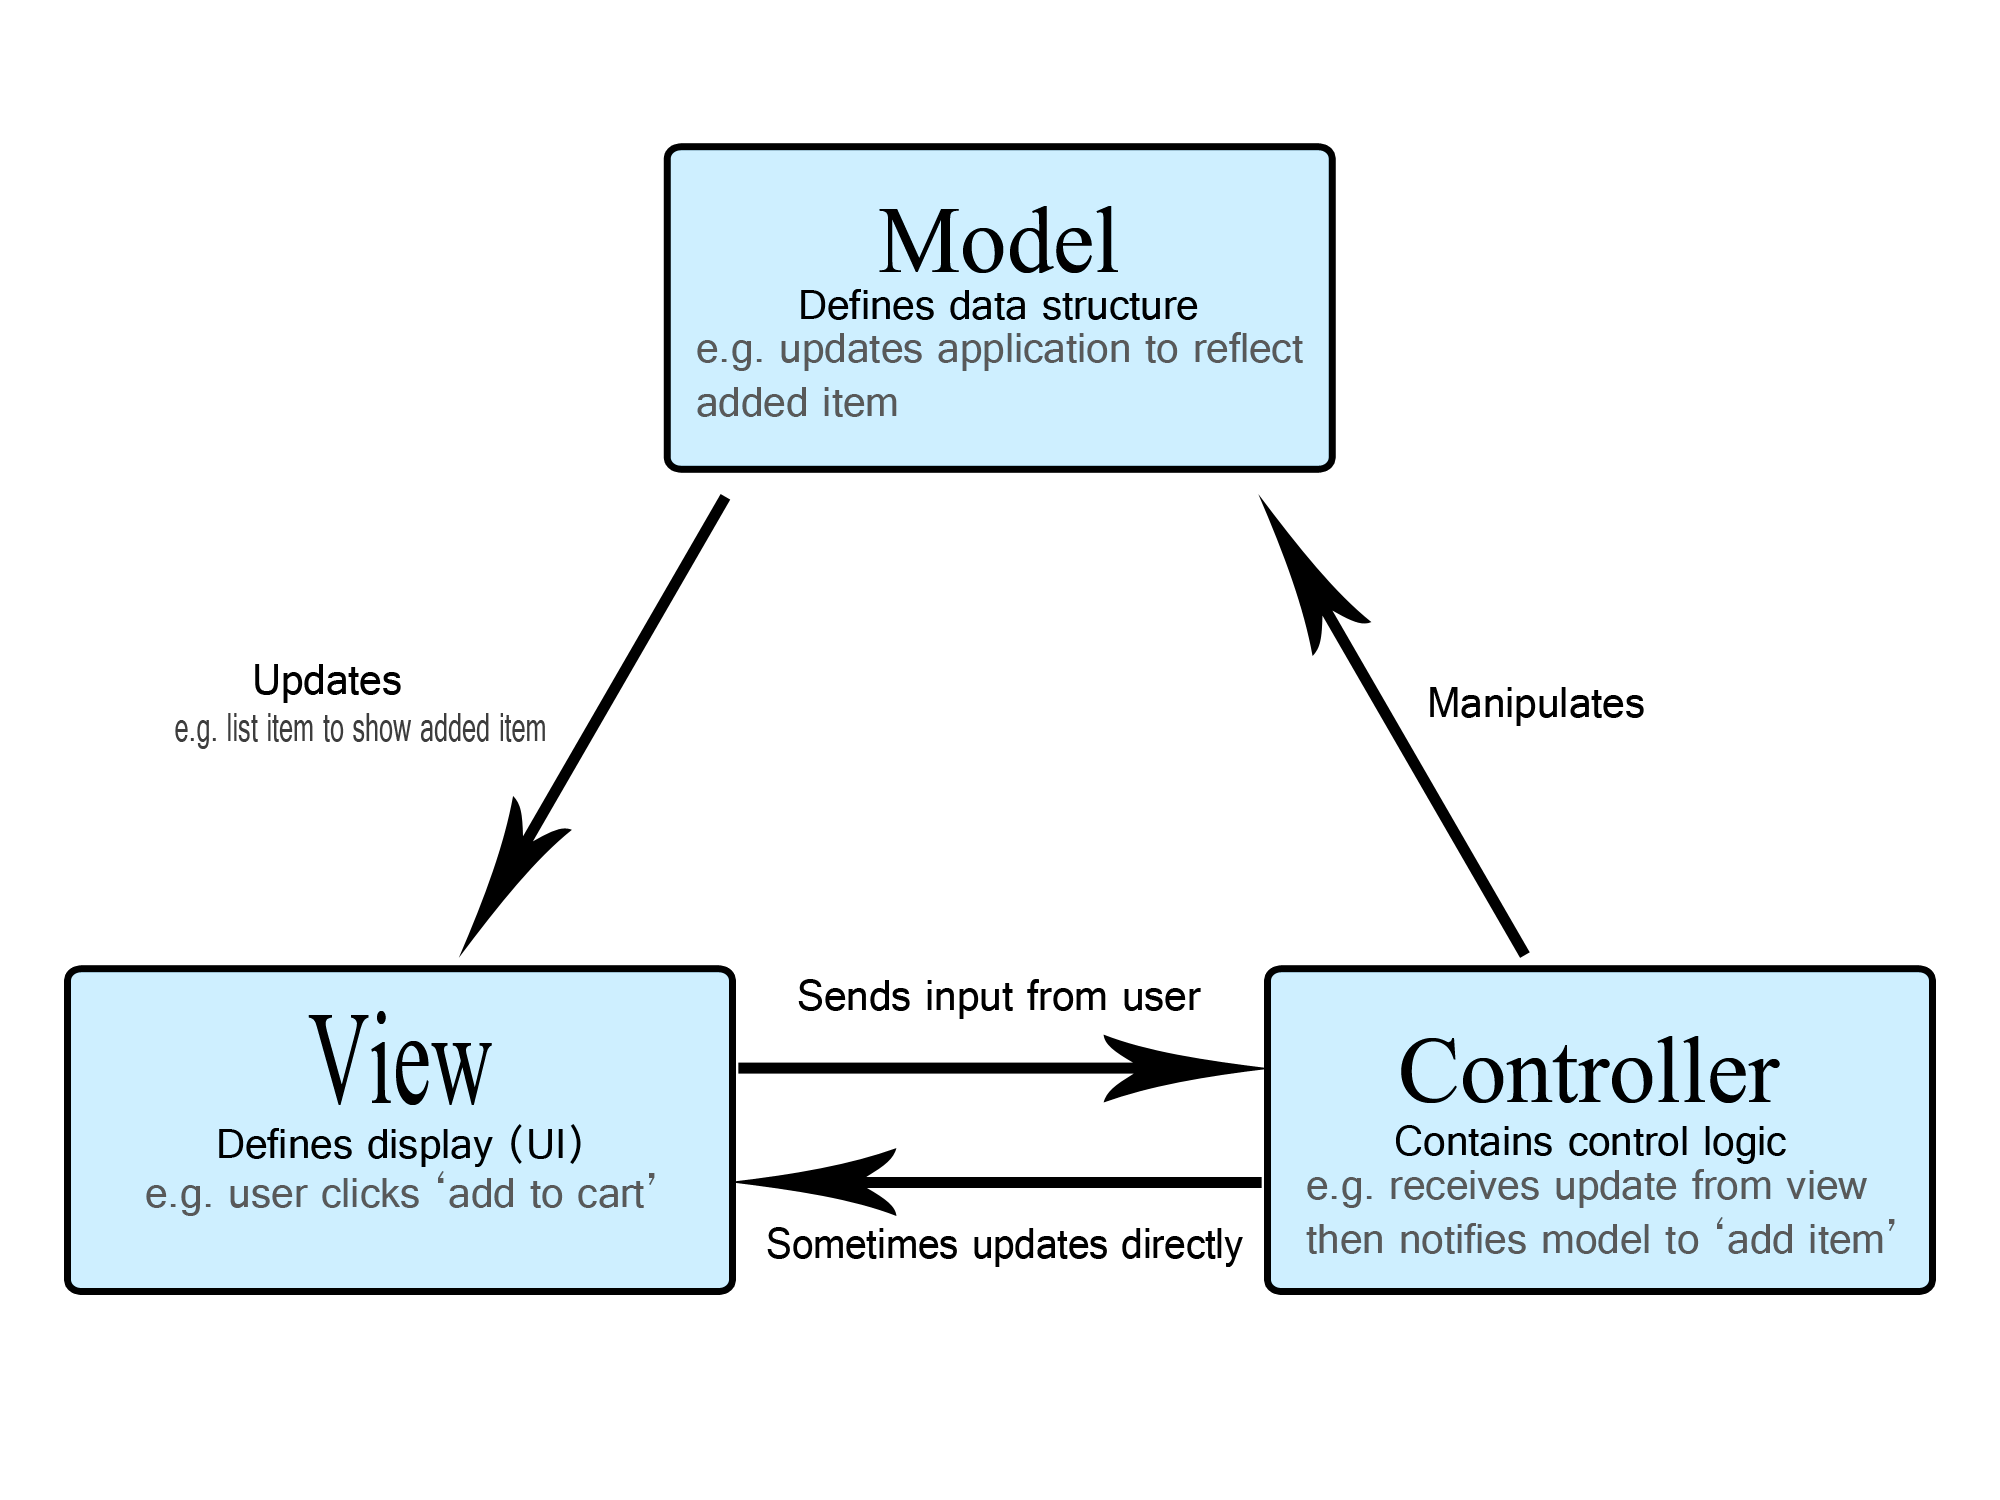
\includegraphics[scale=0.55]{img/model_view_controller}
	\caption{Model-View-Controller Entwurfsmuster} 
	\footnotesize\sffamily\textbf{Quelle:} \url{https://developer.mozilla.org/en-US/docs/Glossary/MVC}
	\label{fig:mvc}
  \end{center}   
\end{figure}

Durch die nicht mehr so starke Kopplung der Komponenten, gewährleistet das MVC-Entwurfsmuster eine höhere Flexibilität im Programmdesign. Außerdem hat Herr Steffen D. in seinem Blog folgende Vorteile über das MVC-Entwurfsmuster aufgeführt:\bigskip

\par
\begingroup
\leftskip=4em % Parameter anpassen
\rightskip\leftskip
\noindent \glqq Vorteile finden sich zum einen in der Möglichkeit, dass ein und dasselbe Datenmodell in mehreren Ansichten repräsentiert werden kann. Des Weiteren sind alle Ansichten, die sich auf ein Modell beziehen, automatisch synchronisiert und es können Bedienelemente beliebig vertauscht werden. Außerdem ist es ohne Weiteres möglich auf einem vorhandenen Modell einen neuen View zu implementieren. Dadurch ist ein solches System nahezu beliebig skalierbar.\grqq{} \cite{Stef2018}
\par
\endgroup
\bigskip

\newpage
Die \textbf{Abbildung \ref{fig:mvc_anwendung}} stellt das MVC-Entwurfsmuster der zu realisierenden Webanwendung dar. Die WebSockets-Komponente kommuniziert sowohl mit der View als auch mit dem Controller. Im Controller wird die Anwendungslogik des WebSockets implementiert. Mit Hilfe des WebSockets werden auf der View-Komponente anschließend die Anwendungsdaten in Echtzeit präsentiert.\bigskip

\begin{figure}[H]
  \begin{center}
    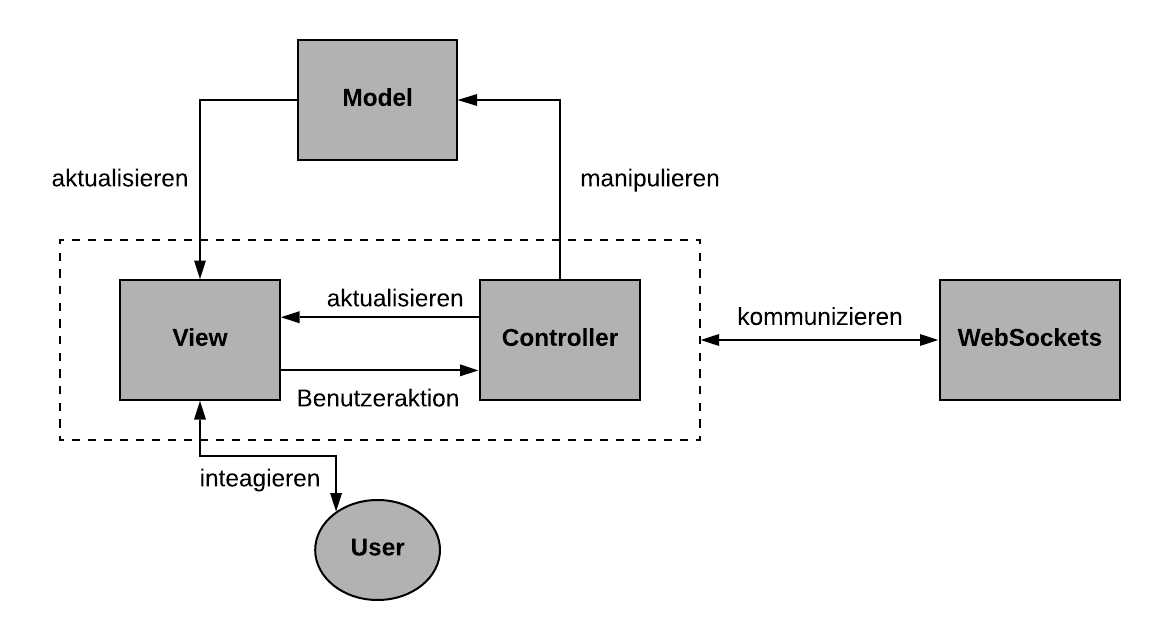
\includegraphics[scale=0.55]{img/blank_diagramm}
	\caption{Das MVC-Entwurfsmuster angepasst an die zu realisierenden Anwendung} 
	\footnotesize\sffamily\textbf{Quelle:} eigene Abbildung
	\label{fig:mvc_anwendung}
  \end{center}   
\end{figure}

Die \textbf{Abbildung \ref{fig:web architektur}} zeigt die einzelnen Schichten der Model-, Controller-,  und View-Module. In der View-Schicht befinden sich die Views der einzelnen Seiten der Webanwendung. Jede View hat einen eigenen Controller. Zusammen bilden sie ihre eigene Benutzeroberfläche der Webanwendung. Der WebSocket ist hauptverantwortlich für die bidirektionale Kommunikation zwischen der View- und Controller-Schicht. Die Model-Schicht definiert die Datenbankschnittstelle der Anwendung und stellt die Operationen zur Datenmanipulation bereit.

\begin{figure}[H]
  \begin{center}
    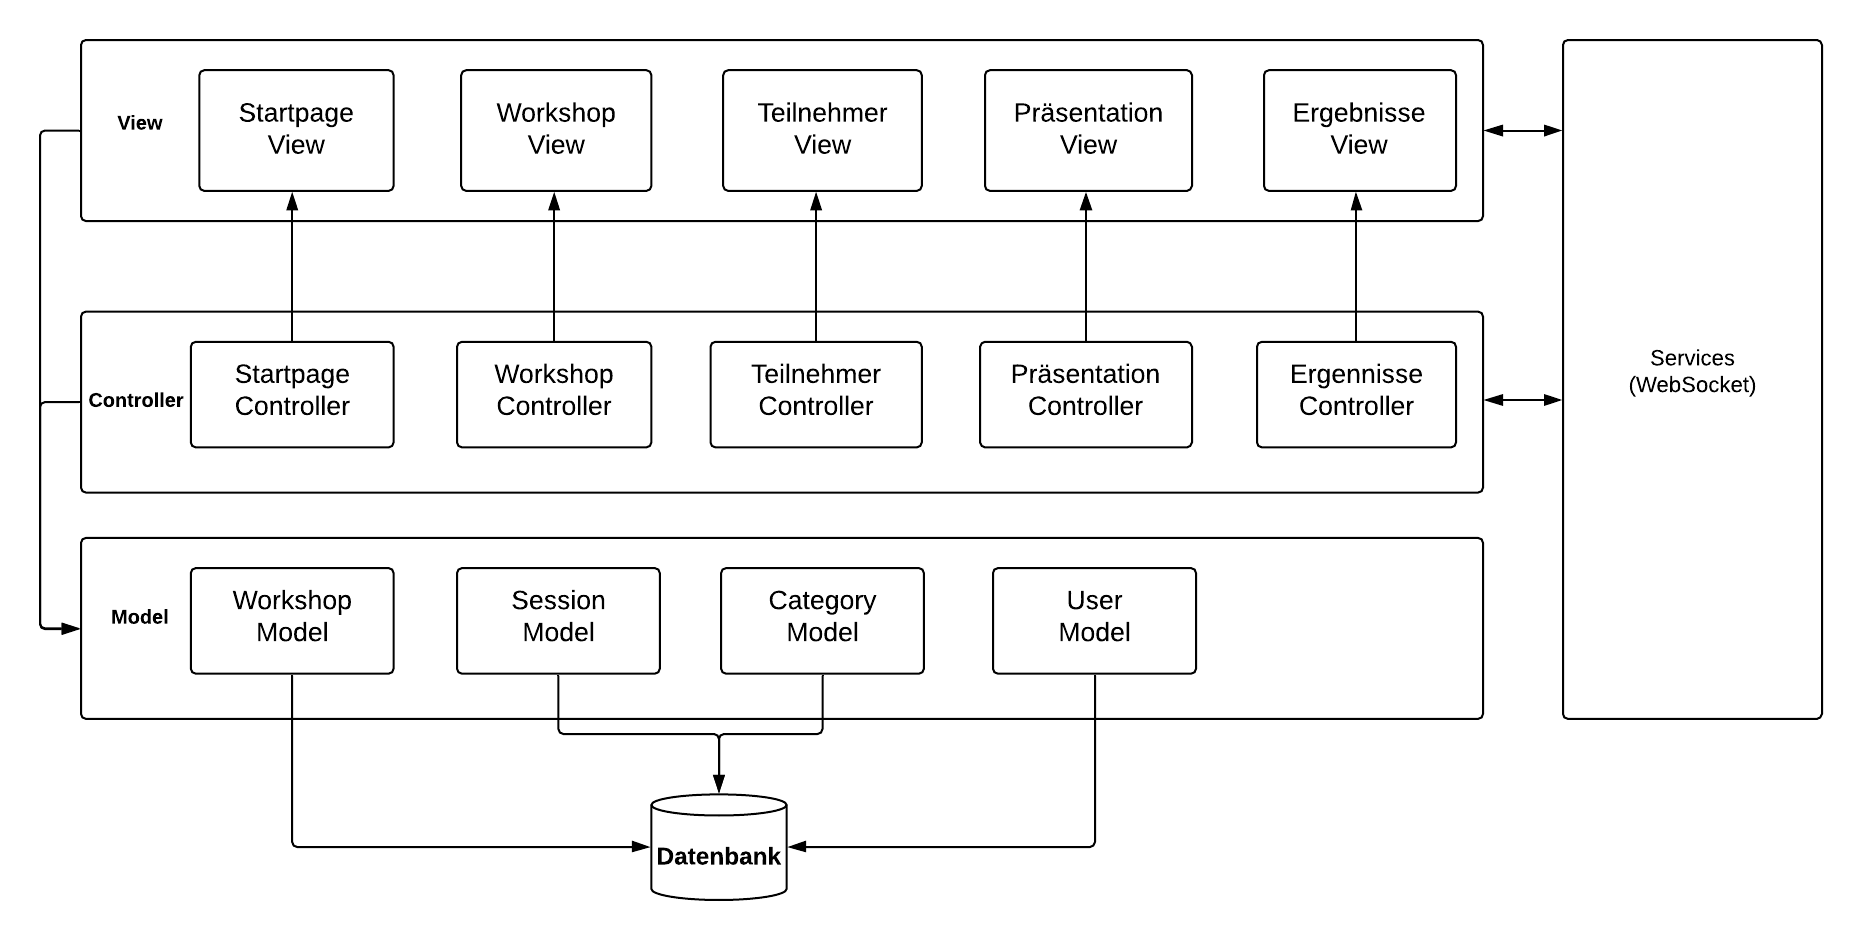
\includegraphics[scale=0.4]{img/web_architektur}
	\caption{Architektur der Webanwendung} 
	\footnotesize\sffamily\textbf{Quelle:} eigene Abbildung
	\label{fig:web architektur}
  \end{center}   
\end{figure}

\section{Serverseitige Implementierung}
\label{sec:Serverseitige Implementierung}
Die Serverapplikation wurde mit der WebSocket-Bibliothek namens Ratchet, welche schon im \textbf{Abschnitt \ref{subsce:Ratchet und Autobahn|JS}} erläutert wurde, umgesetzt. Der WebSocket-Server fungiert in dieser Webanwendung als Router, der die Informationen von einem Client zu anderen Clients in Echtzeit transferiert. Das \textbf{Listing \ref{lst:websocket-server}} stellt den WebSocket-Server dar, welcher in php implementiert wurde. Diese php-Datei muss vor jeder Anwendung ausgeführt werden, um den Server zu starten. Der Server ist über die IP-Adresse 127.0.0.1 und den Port 7070 aufrufbar. Damit die Clients die WebSockets-Verbindung aufbauen können, muss auf der Clientseite das Protokoll \glqq ws\grqq{}, die Adresse und der Port angegeben werden. Die Server-Adresse auf der Clientseite lautet somit \glqq ws://127.0.0.1:7070\grqq{}.\bigskip

\begin{lstlisting}[caption={WebSocket-Server - php}, label=lst:websocket-server, captionpos=b]
use Thruway\Peer\Router;
use Thruway\Transport\RatchetTransportProvider;

//Erzeugt neuer Router mit der Adresse 127.0.0.1 und den Port 7070
$router = new Router();
$transportProvider = new RatchetTransportProvider("127.0.0.1", 7070);
$router->addTransportProvider($transportProvider);
//Start den Router
$router->start();
\end{lstlisting}

\newpage
\section{Clientseitige Implementierung}
\label{sec:Clientseitige Implementierung}
In diesem Unterkapitel wird die clientseitige Implementierung und die Vorgehensweise bei der Entwicklung der Webanwendung beschrieben.\bigskip

\begin{figure}[H]
  \begin{center}
    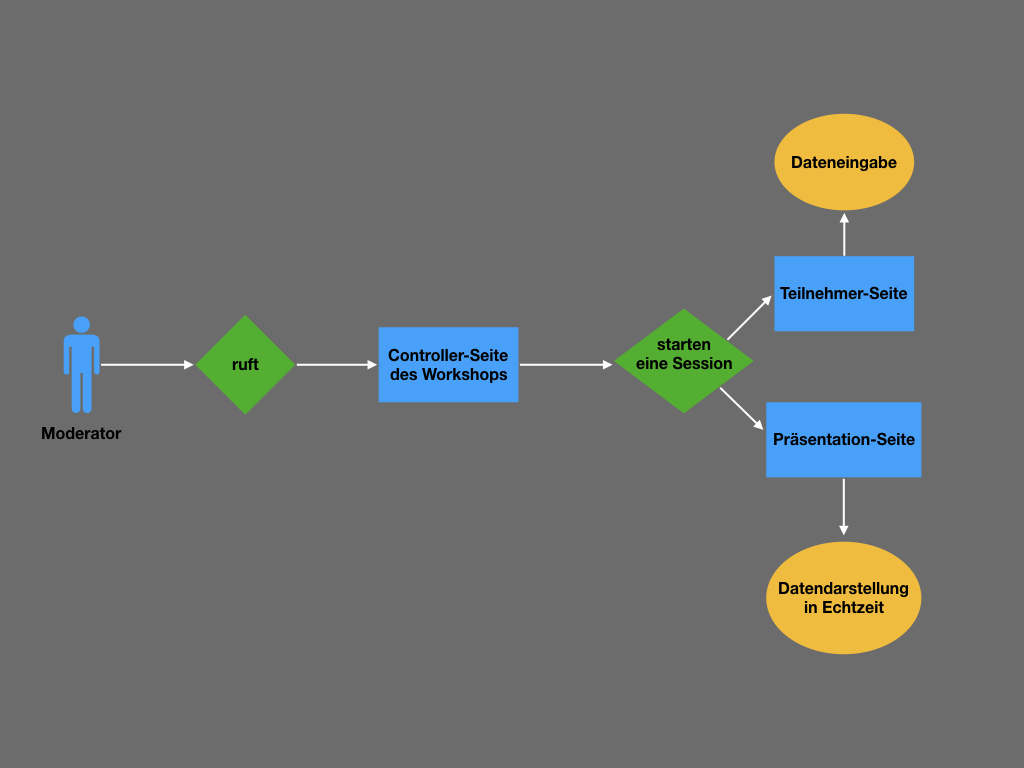
\includegraphics[scale=0.35]{img/Workflow_controllerSeite}
	\caption{Workflow auf der Controller-Seite} 
	\footnotesize\sffamily\textbf{Quelle:} eigene Abbildung
	\label{fig:workflow_controller-seite}
  \end{center}   
\end{figure}

Die \textbf{Abbildung \ref{fig:workflow_controller-seite}} beschreibt den Arbeitsablauf auf der Controller-Seite. Nachdem der Moderator einen Workshop erstellt hat, ruft er diesen auf. Er wird anschließend auf die Controller-Seite des Workshops weitergeleitet.
Der Moderator erstellt für die Ideenfindung eine neue Session und startet sie. Auf der Teilnehmer-Seite wird beim Starten der Session die Eingabefunktion freigeschaltet. Auf der Präsentation-Seite wird beim Starten der Session ein Bereich für die Darstellung von Daten bereitgestellt.\bigskip

Um diesen beschriebenen Arbeitsablauf, wie auf der \textbf{Abbildung \ref{fig:workflow_controller-seite}} dargestellt, zu realisieren, kommt das WAMP-Protokoll \textbf{(Abschnitt \ref{sec:wamp})} zum Einsatz. Dabei wird das Publish-Subscribe-Muster (PubSub-Muster) angewendet, bei dem die Abonnenten (Subscribers) die vom Verteiler (Publisher) veröffentlichte Nachrichten empfangen können. Der WebSocket-Server übernimmt beim PubSub-Muster das Nachrichten-Routing, welcher nur eine Aufgabe hat, die veröffentlichten Nachrichten an die Abonnenten zu verteilen \textbf{(Abbildung \ref{fig:workflow_mit_websocket_controller_seite})}.\bigskip

\begin{figure}[H]
  \begin{center}
    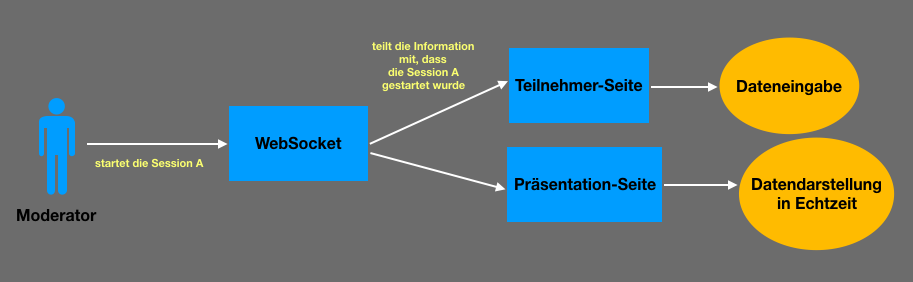
\includegraphics[scale=0.4]{img/workflow_mit_websocket_controller_seite}
	\caption{PubSub-Protokoll} 
	\footnotesize\sffamily\textbf{Quelle:} in Anlehnung an \url{https://blog.felix-seifert.com/web-application-messaging-protocol/}
	\label{fig:workflow_mit_websocket_controller_seite}
  \end{center}   
\end{figure}

Der WebSocket-Server wurde bereits im vorherigen Unterkapitel implementiert. Nun wird jeweils auf der Controller-, Teilnehmer- sowie Präsentation-Seite eine Verbindung zum WebSocket-Server aufgebaut. Als Werkzeug für die Implementierung kommt das AutobahnJS \textbf{(Abschnitt \ref{subsce:Ratchet und Autobahn|JS})} zum Einsatz.\bigskip

Das \textbf{Listing \ref{lst:verbindungsaufbau zum websocket-server}} zeigt, wie eine Verbindung zum WebSocket-Server aufgebaut wird. Die URL gibt die Adresse zum WebSocket-Server an, welcher das Protokoll \glqq ws\grqq{} verwendet. Der \glqq realm\grqq{}-Parameter legt eine Domäne oder einen Bereich für das Nachrichten-Routing fest. Es ist zu beachten, dass die Abonnenten die veröffentlichten Nachrichten empfangen können, wenn sie im selben Bereich wie der Herausgeber (Publisher) sind.\bigskip 

\begin{lstlisting}[caption={Verbindungsaufbau zum WebSocket-Server - php}, label=lst:verbindungsaufbau zum websocket-server, captionpos=b]
var connection = new autobahn.Connection({
       url: "ws://127.0.0.1:7070",
       realm: "workshoppy"
   });
\end{lstlisting}

\newpage
\subsection{Session starten}
\label{Session starten}
Die Session ist erst gestartet, wenn der \glqq Session starten\grqq{}-Button auf der Controller-Seite getätigt wird \textbf{(Abbildung \ref{fig:controller-Seite final})}.\bigskip

\begin{figure}[H]
  \begin{center}
    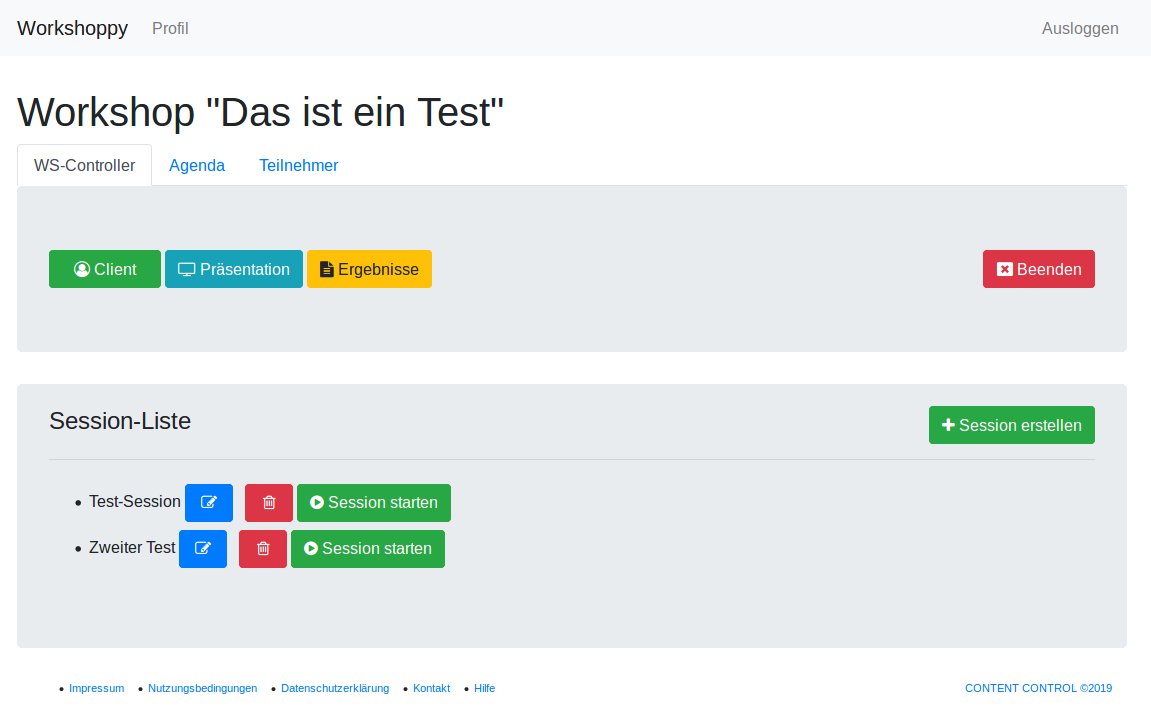
\includegraphics[scale=0.3]{img/controller-seite_real}
	\caption{Controller-Seite} 
	\footnotesize\sffamily\textbf{Quelle:} eigene Abbildung
	\label{fig:controller-Seite final}
  \end{center}   
\end{figure}

Die Implementierung auf der Controller-Seite erfolgt mittels JavaScript \textbf{(Listing \ref{lst:Publish-Muster Controller-Seite})}. Die Variable \glqq controller\_topic\grqq{} beschreibt die URI des Workshops, über die eine Ressource identifiziert wird.\bigskip 

Innerhalb der \glqq add\_controls\grqq{}-Funktion wurde ein Event-Handler für den \glqq Session starten\grqq{}-Button implementiert. Ein Event (Ereignis) wird ausgelöst, wenn der Button geklickt wird. Das id-Attribut \glqq session-list\grqq{} gibt den Bereich an, in dem sich der Button befindet. Das Button-Element selbst wird über das class-Attribut \glqq session-start\grqq{} angesprochen. Mit dem onclickt-Event wird dabei eine Funktion aufgerufen. In dieser Funktion wurde das Publish-Muster für die Verteilung der Nachrichten implementiert. Es wird dabei ein Objekt mit zwei Werten an die Abonnenten gesendet. Der Schlüssel \glqq stage\grqq{} mit dem Wert \glqq session\grqq{} gibt an, dass die Session gestartet ist. Auf die Session-Frage kann über den Schlüssel \glqq msg\grqq{} zugegriffen werden. Das Event-Listener \glqq connection.onopen\grqq{} indiziert, dass die Verbindung mit dem WebSocket-Server bereit ist, so dass man Informationen versenden und empfangen kann. Bei einem Verbindungsfehler oder wenn die Verbindung zum WebSocket geschlossen ist, wird auf der Konsole eine Warnung ausgegeben.

\newpage
\begin{lstlisting}[caption={Publish-Muster auf der Controller-Seite - JavaScript}, label=lst:Publish-Muster Controller-Seite, captionpos=b]
//URI von Controller-Seite
var controller_topic = 'de.ccb.workshoppy.controller.' + window.workshoppy.guid;
//Verbindung ist geöffnet
connection.onopen = function(session, details) {
   add_controls(session);
};
//Verbindung ist geschlossen
connection.onclose = function (reason, details) {
//Warnungausgabe
   console.warn('WebSocket connection closed: ' + reason);
};
function add_controls(session) {
//clickt-Event für den Session starten Button
  $('#session-list').on('click', '.session-start', function(e) {
//Abonniert die Controller-Seite, um Nachrichten zu empfangen
      session.publish(controller_topic, [{
     	  //Übermittelte Daten
          stage: 'session',
          msg: $(this).attr('data-question');
      }]);
  });
}
\end{lstlisting}

\newpage
Um die Daten vom Publisher (Controller-Seite) empfangen zu können, muss der Empfänger (Teilnehmer-Seite) das Publisher-Event \glqq controller\_topic\grqq{} abonnieren. Diese Vorgehensweise wird mit dem Subscribe-Muster umgesetzt. \textbf{(Listing \ref{lst:Subscribe-Muster Teilnehmer-Seite})}.\bigskip

\begin{lstlisting}[caption={Subscribe-Muster auf der Teilnehmer-Seite - JavaScript}, label=lst:Subscribe-Muster Teilnehmer-Seite, captionpos=b]
//Controller-Event
var controller_topic = 'de.ccb.workshoppy.controller.' + window.workshoppy.guid,
  //Teilnehmer-Event
    client_topic = 'de.ccb.workshoppy.client.' + window.workshoppy.guid;
//Stellt eine Verbindung zum WebSocket-Server her
var connection = new autobahn.Connection({
    url: "ws://127.0.0.1:7070",
    realm: "workshoppy"
   });
//Verbindung ist geöffnet
connection.onopen = function(session, details) {
	//Abonniere der Controller-Seite, um Nachrichten zu empfangen
      session.subscribe(controller_topic, function(args) {
	//Aktualisiere die Eingabefunktion auf der Teilnehmer-Seite
          update_stage(args[0]);
      });
	//Funktion für das Abschicken der Daten
      add_controls(session);
}
//Verbindung ist geschlossen
connection.onclose = function (reason, details) {
	//Warnungausgabe
	console.warn('WebSocket connection closed: ' + reason);
};
\end{lstlisting}

\newpage
Die Funktion \glqq update\_stage\grqq{}” im Subscribe-Muster im \textbf{Listing \ref{lst:Subscribe-Muster Teilnehmer-Seite}} stellt die Eingabefunktion auf der Teilnehmer-Seite (Abbildung 5.x: Teilnehmer-Seite) zur Verfügung, wenn das empfangene Objekt (data) den Zustand \glqq session\grqq{} aufweist \textbf{(Listing \ref{lst:update-stage})}.

\begin{lstlisting}[caption={Stellt die Eingabefunktion auf der Teilnehmer-Seite bereit - JavaScript}, label=lst:update-stage, captionpos=b]
function update_stage(data) {
	//Das empfangene Objekt wird geprüft
	if (data.stage === 'session') {
		//Wählt ein Element mit dem angegebenen id-Attribut aus und fügt die Session-Frage hier ein.
		$('#question').text(data.msg);
		//Gib der Bereich zur Dateneingabe frei
		$('#stage-session').show();
       }
   }
\end{lstlisting}

Das \textbf{Listing \ref{lst:html client}} beschreibt die HTML-Struktur der Teilnehmer-Seite \textbf{(Abbildung \ref{fig:teilnehmer-Seite final})}. Innerhalb des <form>-Tags befindet sich das gesamte Formular (Textarea und Button) für die Dateneingabe. Die Session-Frage, welche eine Überschrift zweiter Ordnung ist, wurde mittels Heading-Tag (<h2></h2>) definiert.\bigskip

\begin{lstlisting}[caption={HTML-Struktur der Teilnehmer-Seite}, label=lst:html client, captionpos=b]
<div class="container stage" id="stage-session">
    <h2 id="question" class="text-center"></h2>
    <hr class="my-4">
    <form id="answer">
        <div class="form-group row">
            <div class="col-sm-12">
                <textarea rows="4" cols="56" id="message_input" required
                    class="form-control"
                    placeholder="Bitte gib deine Antwort ein..."></textarea>
            </div>
        </div>
        <button class="btn btn-primary btn-block" type="submit">
            <i class="fa fa-comment" aria-hidden="true"></i>
            Abschicken
        </button>
    </form>
</div>
\end{lstlisting}

\begin{figure}[H]
  \begin{center}
    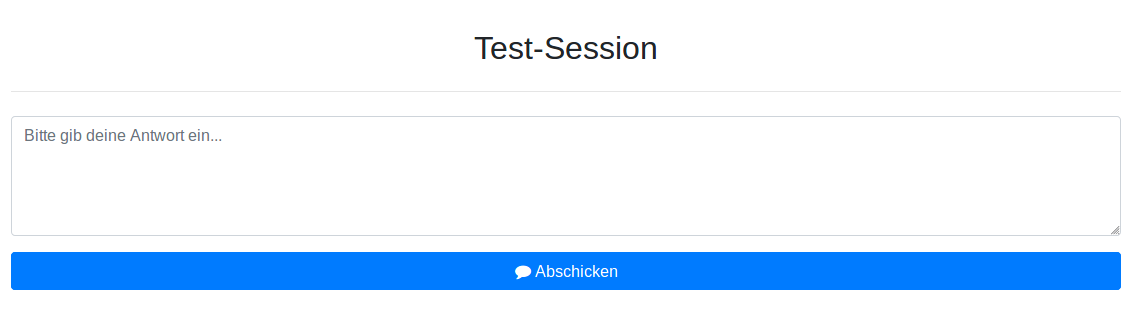
\includegraphics[scale=0.35]{img/client}
	\caption{Teilnehmer-Seite} 
	\footnotesize\sffamily\textbf{Quelle:} eigene Abbildung
	\label{fig:teilnehmer-Seite final}
  \end{center}   
\end{figure}

\subsection{Dateneingabe auf der Teilnehmer-Seite}
\label{subsec:Dateneingabe auf der Teilnehmer-Seite}
Das \textbf{Listing \ref{lst:abschicken der daten}} beschreibt die \glqq add\_controls\grqq{}-Funktion im \textbf{Listing \ref{lst:Subscribe-Muster Teilnehmer-Seite}}. Diese Funktion sorgt auf der Teilnehmer-Seite dafür, dass die Daten nach dem Tätigen des Abschicken-Buttons bei der Präsentation-Seite ankommen. Das Eingabeformular wird in einem form-Tag definiert \textbf{(Listing \ref{lst:html client})}. Das Button-Element ist vom typ-Attribut \glqq submit\grqq{}, welches beim Klicken auf den Button ein submit-Event auslöst. Innerhalb der Funktion des submit-Events wird das Publish-Muster für die Verbreitung der eingegeben Daten implementiert. Über die Variable \glqq client\_topic\grqq{} im \textbf{Listing \ref{lst:Subscribe-Muster Teilnehmer-Seite}} wird die Teilnehmer-Seite (Publisher) identifiziert. Die Daten werden als ein Objekt (cardData) übermittelt. In diesem Objekt sind der Name des Absenders und seine eingegeben Daten enthalten. \bigskip

\begin{lstlisting}[caption={Funktion für das Abschicken von Daten auf der Teilnehmer-Seite - JavaScript}, label=lst:abschicken der daten, captionpos=b]
function add_controls(session)
	//Submit-Event
	$('#answer').on('submit',function(e) {
		//Wenn der Benutzername leer ist, wird eine Meldung ausgegeben, dass der Benutzername eingegeben werden muss.
		if (typeof username === 'undefined'){
        		alert("Username muss gesetzt werden");
            return;
   		}
		//Die Variable 'msg' wird mit den eingegebenen Daten initialisiert.
		var msg = $(this).find('textarea').val(),
		//Daten sowie Benutzernamen werden in einem Objekt gespeichert.
			cardData = {
            		'user_id': username,
            		'msg': msg
            },
		//Verbreite die Nachricht an seine Abonnenten
		session.publish(client_topic, [cardData]);
		$(this).find('').val('').focus();
		$(this).find('textarea').val('').focus();
	});
\end{lstlisting}

Die Teilnehmer-Seite übernimmt im Prinzip zwei Rollen:
\begin{enumerate}
\item der Subscriber, der die Nachrichten von der Controller-Seite empfängt.
\item der Publisher, der die eingegebenen Daten der Teilnehmer an die Präsentation-Seite weiterleitet.
\end{enumerate}

\subsection{Darstellung von Daten in Echtzeit}
\label{subsce:Darstellung von Daten in Echtzeit}
Die Präsentation-Seite ist das Herzstück der Webanwendung. Auf dieser werden die eingegebenen Daten von den Teilnehmern in Echtzeit dargestellt und anschließend werden die gesammelten Daten in Kategorien zusammengefasst. Damit die Präsentation-Seite die Daten in Echtzeit darstellen kann, muss zunächst eine Verbindung zum WebSockets-Server aufbaut werden (vgl. \textbf{Listing \ref{lst:verbindungsaufbau zum websocket-server}}).\bigskip

Die Präsentation-Seite muss den \glqq client\_topic\grqq{} abonnieren, um die Nachrichten der Teilnehmer empfangen zu können \textbf{(Listing \ref{lst:subscribe auf der Präsentation-Seite})}.\bigskip

\begin{lstlisting}[caption={Subscribe-Muster auf der Präsentation-Seite - JavaScript}, label=lst:subscribe auf der Präsentation-Seite, captionpos=b]
//Verbindung zum WebSocket ist geöffnet
connection.onopen = function(session, details) {
	//Abonniere die Teilnehmer-Seite, um die eingegebenen Daten zu erhalten
	session.subscribe(client_topic, function (args) {
		//Funktion zur Darstellung der Daten
    		add_card(args[0]);
	});
};
\end{lstlisting}

Die Funktion \glqq add\_card\grqq{}, welche im \textbf{Listing \ref{lst:subscribe auf der Präsentation-Seite}} zu sehen ist, wird im \textbf{Listing \ref{lst:add_card}} detailliert vorgestellt. Die empfangenen Daten werden wie eine Karte auf der Präsentation-Seite dargestellt. Auf dieser Karte sind der Benutzername (user\_id) und dahinter die Nachricht (msg) zu sehen. Als Gestaltungsvorlage werden die Klasse \glqq alert\grqq{} und \glqq alert-warning\grqq{} vom Bootstrap verwendet. Die Daten werden in einem Array namens \glqq cards\grqq{} gespeichert. Mit Hilfe der JQuery-Methode \glqq append\grqq{} werden die Daten im Bereich \glqq message\_output\grqq{} auf der Präsentation-Seite dargestellt \textbf{(Abbildung \ref{fig:Präsentation-Seite final})}.\bigskip

\begin{lstlisting}[caption={Funktion zur Visualisieren der Daten auf der Präsentation-Seite - JavaScript}, label=lst:add_card, captionpos=b]
function add_card(data) {
	var card = $('<div data-index="' + index +'" class="alert alert-warning"><p><b>' + htmlDecode(data.user_id) + ':</b> ' + htmlDecode(data.msg) + '</p></div>'),
	//Die Daten werden in einem Arrey namens cards gespeichert
	cards.push(data);
    $('#message_output').append(card);
}
\end{lstlisting}

\begin{figure}[H]
  \begin{center}
    \includegraphics[scale=0.35]{img/präsentation_seite}
	\caption{Präsentation-Seite} 
	\footnotesize\sffamily\textbf{Quelle:} eigene Abbildung
	\label{fig:Präsentation-Seite final}
  \end{center}   
\end{figure}

\newpage
\subsection{Daten in Kategorien zusammenfassen}
\label{subsec:Daten in Kategorien zusammenfassen}
Die auf der Präsentation-Seite befindlichen Daten können erst in Kategorien zusammengefasst werden, wenn die Ideensammlungsphase vorüber ist. Das bedeutet, dass der \glqq Eingabe beenden\grqq{}-Button auf der Controller-Seite getätigt werden muss \textbf{(Abbildung \ref{fig:controller-Seite mit session final})}. Durch das Klicken auf diesen Button wird auf der Präsentation-Seite ein neuer Button namens \glqq Kategorien erstellen\grqq{} eingeblendet und die Eingabe auf der Teilnehmer-Seite wird dabei gestoppt. Es können demzufolge keine weiteren Daten mehr eingegeben werden. 

\bigskip
\begin{figure}[H]
  \begin{center}
    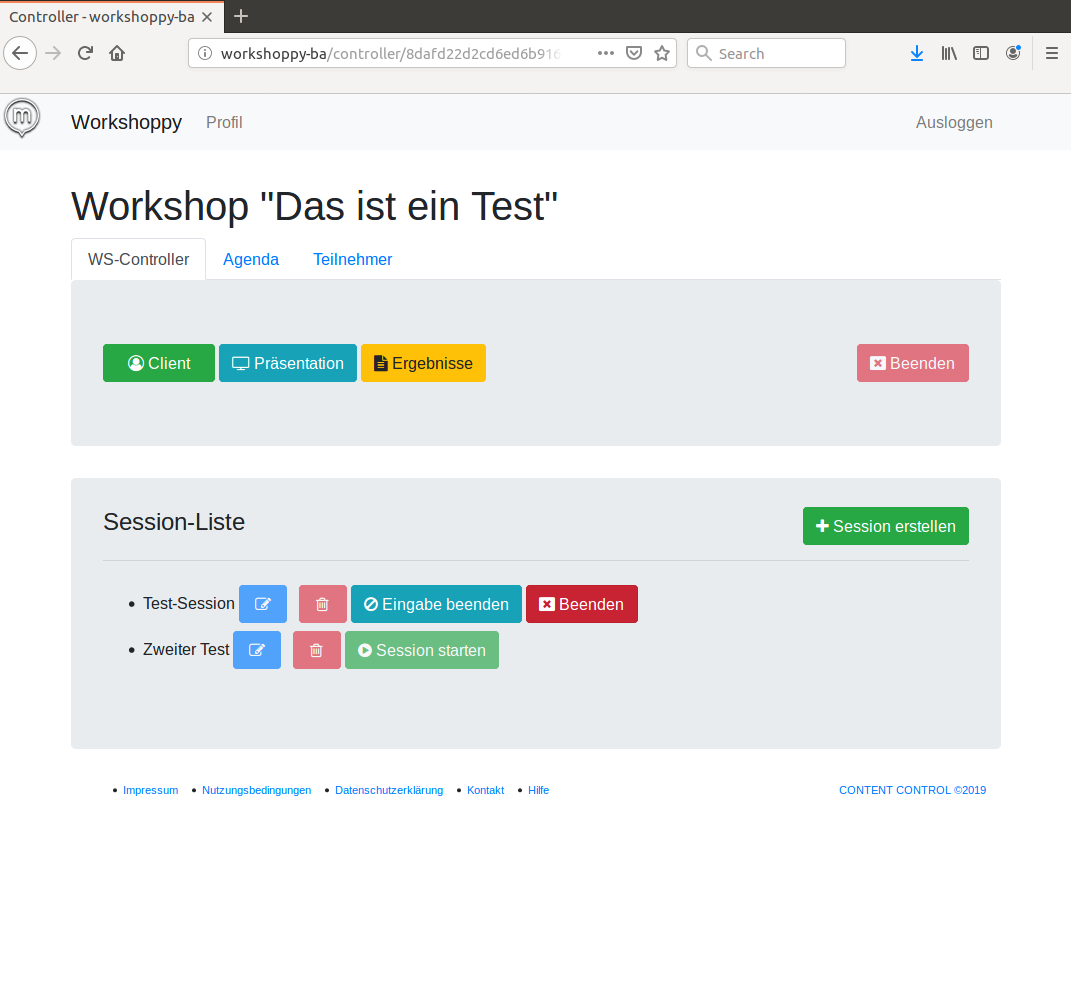
\includegraphics[scale=0.35]{img/controller_seite1}
	\caption{Controller-Seite, wenn die Session gestartet ist} 
	\footnotesize\sffamily\textbf{Quelle:} eigene Abbildung
	\label{fig:controller-Seite mit session final}
  \end{center}   
\end{figure}

\newpage
Das \textbf{Listing \ref{lst:html präsentation-seite}} stellt den Aufbau des Inhaltsbereiches auf der Präsentation-Seite dar. Bei der Session-Frage handelt es sich, wie auf der Teilnehmer-Seite, um eine Überschrift zweiter Ordnung. Die eingegebenen Daten befinden sich innerhalb des div-Elements mit der Id \glqq message\_output\grqq{}. Das div-Element ist ein Bereich, in welchem Elemente eingeschlossen werden. Die erstellten Kategorien werden im Bereich \glqq category\_output\grqq{} dargestellt. Der Titel einer Kategorie kann durch das Anklicken auf den Bereich \glqq Kategorie-Titel\grqq{} verändert werden. Die Kategorie wurde mit Hilfe von JavaScript umgesetzt, wie im \textbf{Listing \ref{lst:kategorie umsetzen}} zu sehen ist. Gespeichert werden sie in einem Array namens \glqq categories\grqq{}. Über das Id-Attribut werden die Kategorien angesprochen.\bigskip

\begin{lstlisting}[caption={HTML-Struktur der Präsentation-Seite}, label=lst:html präsentation-seite, captionpos=b]
<div class="container-fluid stage" id="stage-session">
	<h2 id="question" class="text-center"></h2>
    <hr class="my-4">
    <div id="message_output"></div>
    <div id="category_output"></div>
</div>

\end{lstlisting}
\bigskip

\begin{lstlisting}[caption={Kategorie umsetzen - JavaScript}, label=lst:kategorie umsetzen, captionpos=b]
function add_category(data) {
	//Kategorie-Titel
	var categoryTitle = $('<div class="row"><div id="categoryTitle-' + data.id + '" class="col categoryTitle" data-category="' + data.id + '">' + htmlDecode(data.title) + '</div></div>'),
	//Kategorie-Body
	categoryBox = $('<div data-category="' + data.id + '" class="connectedSortable sortedMessages"></div>'),
	//Close-Button
	closeButton = $('<a class="boxclose" data-dialog="delete" data-form-id="confirm-delete"</a>'),
	//Trennlinie zwischen Kategorie-Titel und Kategorie-Body
	lineal =  $('<hr class="style1">'),
	//Setzt die Kategorie-Elemente zusammen
	$('#category_output').append(categoryBox);
	categoryBox.append(categoryTitle);
	categoryBox.append(closeButton);
	categoryBox.append(lineal);
	//Speichert die Ids von Kategorien in einem Array namens categories
	categories.push(data);
	//Sortable Funktion
	initSortable(data.id);
}
\end{lstlisting}
\bigskip

\newpage
Innerhalb der \glqq add\_category\grqq{}-Funktion im \textbf{Listing \ref{lst:kategorie umsetzen}} ist eine Funktion namens \glqq initSortable\grqq{} zu sehen. In dieser Funktion wird das Sortable Widgets von JQuery UI implementiert, um die Daten in Kategorien zusammenfassen zu können \textbf{(Listing \ref{lst:sortierfunktion})}.\bigskip

\begin{lstlisting}[caption={Sortierfunktion auf der Präsentation-Seite - JavaScript}, label=lst:sortierfunktion, captionpos=b]
function initSortable(id) {
	if (!$('#message_output').hasClass('connectedSortable')) {
		// Mache aus der Liste mit der Id 'message_output' eine Sortable-Liste.
		$('#message_output').sortable({
		//Definiere eigenes update-Event. Dieses Event wird ausgelöst, wenn der Benutzer die Sortierung beendet und die DOM-Position geändert hat.
		update: function(event, ui) {
			ui.placeholder.css({visibility: 'visible', border: '2px solid yellow'});
			//Hier beginnt die Iteration durch dem 'cards'-Array, wo die Elemente gespeichert sind.
			cards.forEach(function (item) {
				//Eine neue Eigentschaft (Property) namens 'category' mit dem Wert null wird im Array hinzugefügt. Das bedeutet, dass die Elemente, die sich in dieser Liste 'message_output' befinden, keine Kategorien zugeordnet werden.
				item.category = null;
			});
		},
		//Gibt an, dass die Elemente aus der 'alert'-Klasse sortiert werden darf.
		items: '.alert',
		//Gibt an, dass die Elemente aus der 'disbale-sort'-Klasse nicht sortiert werden darf.
		cancel: '.disable-sort',
		//Um Elemente beispielweise von List A nach List B oder umgekehrt zu sortieren, müssen die Option 'connectWith' angewendet werden. Die Option 'connectWith' sorgt dafür, dass die Listen miteinander verbunden werden.
		connectWith: '.connectedSortable'
		}).disableSelection();
		//Ordnet die Liste 'message_output' eine neue Klasse zu.
		$('#message_output').addClass('connectedSortable');
	}
	
	//Mache die Kategorie mit der 'Id' aus der Klasse 'sortedMessages' eine Sortable-Liste.
	$('[data-category="' + id + '"].sortedMessages').sortable({
		//Gibt an, dass die Elemente aus der 'alert'-Klasse sortiert werden darf.
		items: '.alert',
		//Der Kategorie-Titel darf nicht sortiert werden.
		cancel: '.categoryTitle',
		//Jede erstellte Kategorie wurde zwei Klassen ('sortedMessages' und 'connectedSortable') zugeordnet (vgl. Listing  5.11) Die Option 'connectWith' verbindet die Listen aus der Klasse 'connectedSortable' miteinander. Somit können die Elemente von Liste 'message_output' nach Liste 'sortedMessages' sortiert werden und umgekehrt.
		connectWith: '.connectedSortable',
		//Definiere eigenes update-Event. Dieses Event wird ausgelöst, wenn der Benutzer die Sortierung beendet und die DOM-Position geändert hat.
		update: function(event, ui) {
			ui.placeholder.css({visibility: 'visible', border: '2px solid yellow'});
			//Hier beginnt die Iteration durch dem 'cards'-Array, wo die Elemente gespeichert sind.
			cards.forEach(function (item) {
				//Jedes Item in einer Kategorie bekommt die Id von der entsprechenden Kategorie als neue Werte gespeichert.
				item.category = $(event.target).attr('data-category');
			});
		}
	}).disableSelection();
}
\end{lstlisting}

\newpage
\subsection{QR-Code anzeigen}
\label{subsec:QR-Code anzeigen}
Für das Generieren des QR-Codes wurde als Hilfsmittel das frei verfügbare JavaScript-Plugin qrcode.js\footnote{\url{https://github.com/kazuhikoarase/qrcode-generator/tree/master/js}} von Kazuhiko Arase verwendet und nach Anforderungen angepasst. Um dieses Plugin nutzen zu können, muss es in das entsprechende HTML-Dokument importiert werden.\bigskip

\begin{lstlisting}[caption={Importiere das verwendeten JavaScript-Pluing für das Generieren des QR-Codes}, label=lst:plugin, captionpos=b]
<script type="text/javascript" src="qrcode.js"></script>
\end{lstlisting}
\bigskip

Das \textbf{Listing \ref{lst:html für qr-code}} beschreibt den strukturellen Aufbau für das Anzeigen des QR-Codes auf der Präsentationsseite. Der ganze Inhaltsbereich wird in einem div-Tag eingeschlossen. Bei dem QR-Code handelt es sich hierbei um ein Canvas und wird im div-Bereich mit dem Id-Attribut \glqq qrcode\grqq{} angezeigt. Unter dem QR-Code befindet sich die Beschreibung, die in einem Absatz geschrieben wird.\bigskip

\begin{lstlisting}[caption={HTML-Struktur für das Anzeigen des QR-Codes}, label=lst:html für qr-code, captionpos=b]
<div class="container-fluid stage" id="stage-welcome">
	<h1 class="text-center" id="welcome-message">Willkommen bei Workshoppy</h1>
	<div class="col-sm-12 text-center" id="qrcode"></div>
	<p class="text-center" style="font-size: 20px;">Scannen Sie diesen Code, um am Workshop teilzunehmen.</p>
</div>
\end{lstlisting}
\bigskip

Das \textbf{Listing \ref{lst:qr-code generieren}} beschreibt, wie der QR-Code mit Hilfe des JavaScripts auf der Präsentation-Seite generiert wird.\bigskip
\begin{lstlisting}[caption={Generieren des QR-Codes - JavaScript}, label=lst:qr-code generieren, captionpos=b]
//JQuery integrierte Funktion, die verwendet wird, wenn das Browserfenter seine Größe ändert.
$(window).on('resize', function() {
	//Diese Variable gibt die Url der Teilnehmer-Seite mit dem entsprechenden GUID des Workshops an.
	var url = '<?php echo $url_client; ?>/client/' + window.workshoppy.guid + '/';
	//Entfernt zunächst alle untergeordneten Knoten und Inhalte aus den ausgewählten Elementen.
	$('#qrcode').empty();
	//Passt der QR-Code auf die Größe des Browserfensters an.
	var size = Math.min($('#qrcode').width(), $(window).height() - ($('#qrcode').offset().top + 55));
	//In div-Bereich mit dem Id-Attribut 'qrcode' wird der QR-Code anhand der berechneten Größe generiert und gerendert.
	$('#qrcode').qrcode({width: size, height: size, text: url});
});
\end{lstlisting}

\newpage
\begin{figure}[H]
  \begin{center}
    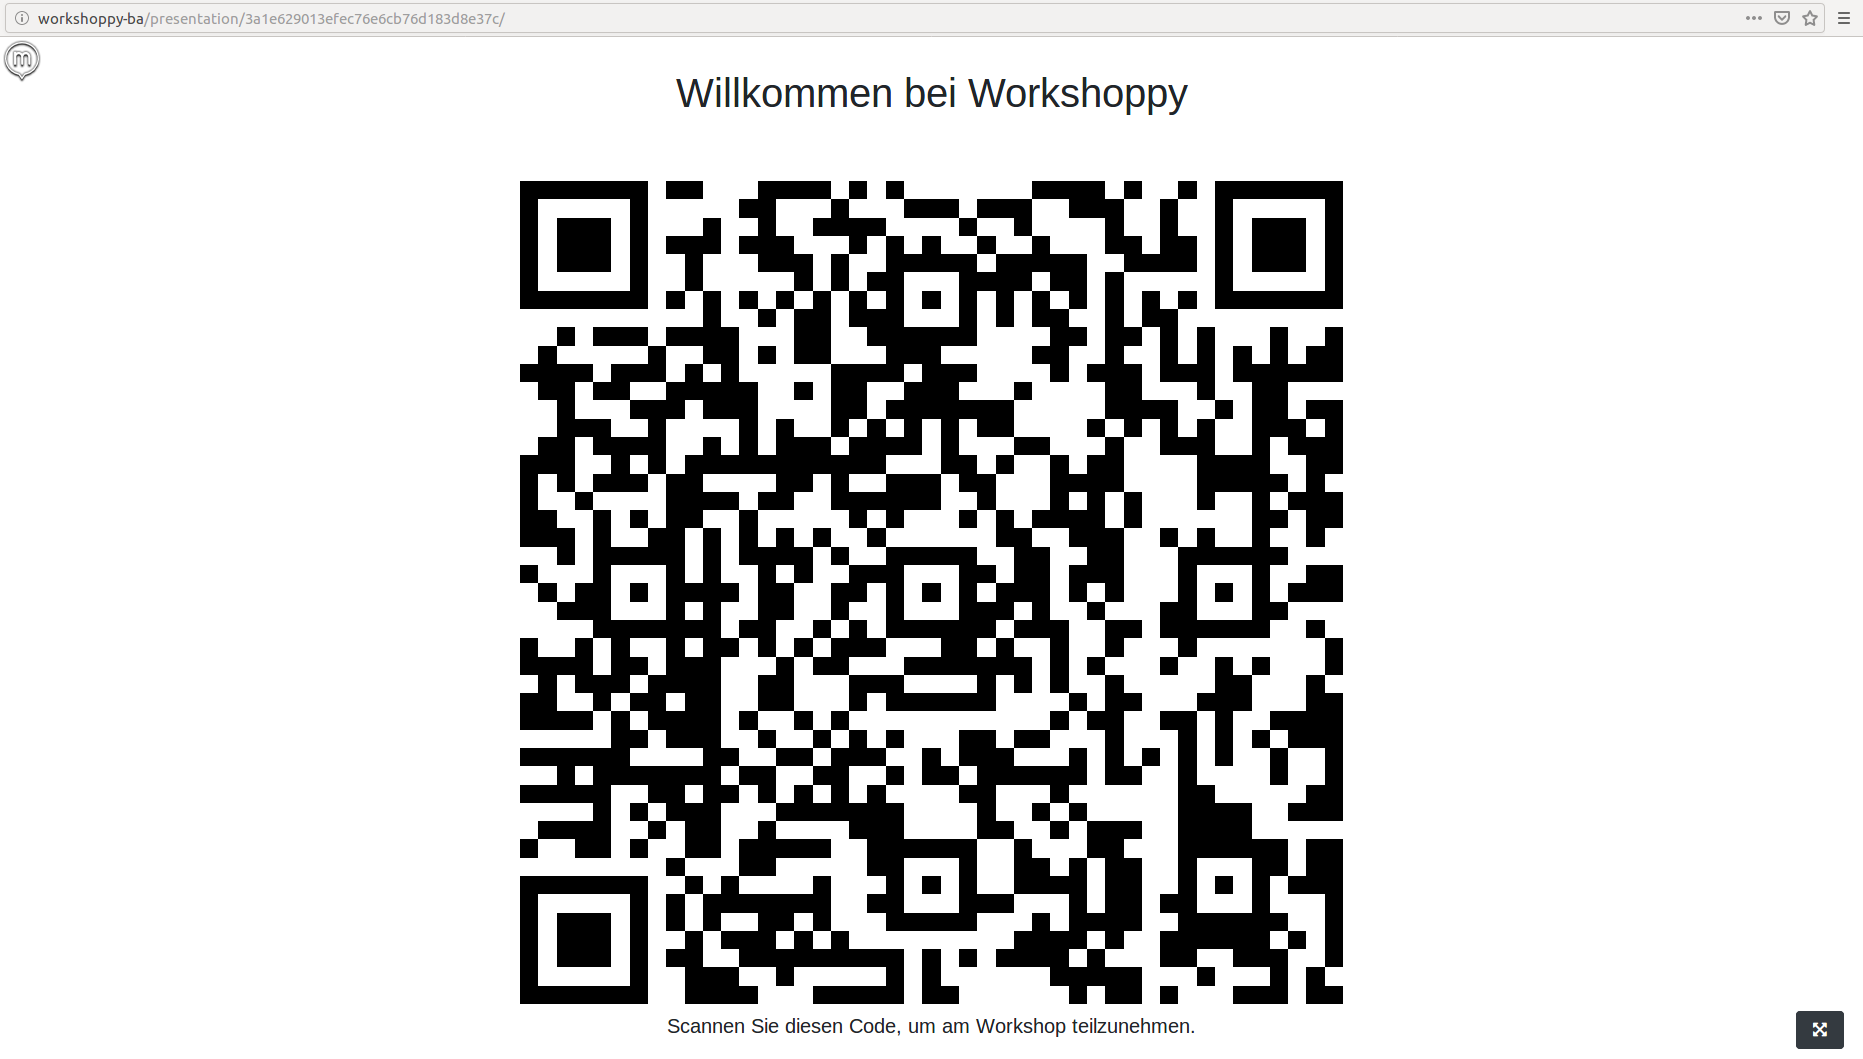
\includegraphics[scale=0.2]{img/qrcode}
	\caption{QR-Code auf der Präsentation-Seite} 
	\footnotesize\sffamily\textbf{Quelle:} eigene Abbildung
	\label{fig:präsentation-seite mit qrcode final}
  \end{center}   
\end{figure}






